\documentclass{beamer}

\usepackage{tikz}
\usepackage{subcaption}
\usetikzlibrary{positioning}
\usepackage[utf8]{inputenc}

\title[] %optional
{Building a Smart Eco-system for Data Centres}

\usetheme{Rochester}
\usecolortheme{default}

\author[Jean Casadedemont] % (optional, for multiple authors)
{Jean Casademont \\ Supervisors: Dr.~Dalal Alrajeh \and Dr.~Luke Dickens}

% \institute[VFU] % (optional)
% {
%   \inst{1}%
%   Faculty of Physics\\
%   Very Famous University
%   \and
%   \inst{2}%
%   Faculty of Chemistry\\
%   Very Famous University
% }

\date[] % (optional)
{23 June 2015}

% \logo{\includegraphics[height=1.5cm]{lion-logo.png}}

\begin{document}

\frame{\titlepage}

\begin{frame}
    \frametitle{Motivations}
    \begin{itemize}
        \item Toward a fully automated cooling system controller.
        \item Model the racks temperature of a datacenter.
        \item Use our model to simulate data and investigate controls.
    \end{itemize}
\end{frame}

\begin{frame}
    \frametitle{Markov Random Fields}
    \begin{columns}
        \column{0.5\textwidth}
        \begin{definition}
            A MRF is a probabilistic graphical model which define a joint distribution of the form:
            $$p = \frac{1}{Z}\prod_{c} \phi_c(c)$$
            where $c$ is a clique in the graph
        \end{definition}
        \begin{example}
            $$p = \frac{ \phi_1(AHU, R_2, R_3) \phi_2(AHU, R_1) }{Z}$$
        \end{example}
        \column{0.5\textwidth}
        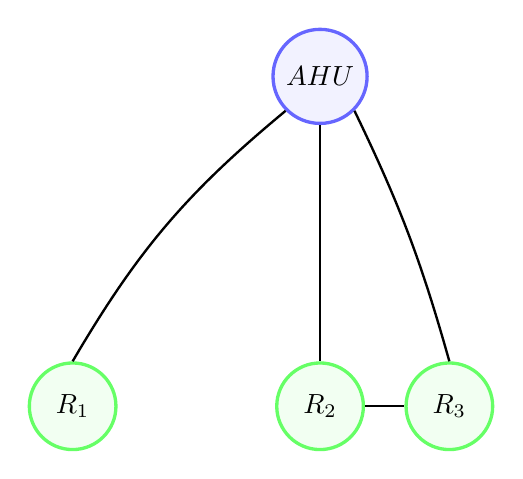
\begin{tikzpicture}[
            racknode/.style={circle, draw=green!60, fill=green!5, very thick, minimum size=1.1cm},
            ahunode/.style={circle, draw=blue!60, fill=blue!5, very thick, minimum size=5mm},
        ]
            %Nodes
            \node[ahunode](ahu){$AHU$};
            \node[racknode](rack1)[below=3cm of ahu] {$R_2$};
            \node[racknode](rack2)[right=0.5cm of rack1] {$R_3$};
            \node[racknode](rack3)[left=2cm of rack1] {$R_1$};

            %Lines
            \draw[line width=0.3mm, -](ahu.south) -- (rack1.north);
            \draw[line width=0.3mm, -](ahu.south west) to [bend right=10] (rack3.north);
            \draw[line width=0.3mm, -](rack1.east) -- (rack2.west);
            \draw[line width=0.3mm, -](ahu.south east) to [bend left=5] (rack2.north);
        \end{tikzpicture}
    \end{columns}
\end{frame}

\begin{frame}
    \frametitle{Gaussian Markov Random Fields}
    \begin{columns}
        \column{0.35\textwidth}
        \begin{itemize}
            \item GMRF is a Pairwise Markov Random Fields
            \item GMRF's joint distribution is a multivariate Gaussian
        \end{itemize}
        \column{0.65\textwidth}
        \begin{figure}
            \includegraphics[scale=0.45]{images/adj_static}
        \end{figure}
    \end{columns}
\end{frame}

\begin{frame}
    \frametitle{GMRF graph}
    \begin{figure}
        \includegraphics<1>[scale=0.45]{images/gmrf_con}
        \includegraphics<2>[scale=0.45]{images/gmrf_adj_qn}
    \end{figure}
\end{frame}

\begin{frame}
    \frametitle{GMRF EO6 predictions}
    \begin{figure}
        \includegraphics[scale=0.7]{images/gmrf_res_eo6}
    \end{figure}
\end{frame}

\begin{frame}
    \frametitle{GMRF Q8 predictions}
    \begin{figure}
        \includegraphics[scale=0.7]{images/gmrf_res_q8}
    \end{figure}
\end{frame}

\begin{frame}
    \frametitle{GMRF QQplot}
    \begin{figure}
        \includegraphics[scale=0.7]{images/simple_gmrf_qqplot}
    \end{figure}
\end{frame}

\begin{frame}
    \frametitle{GMRF Simulation}
    \begin{figure}
        \includegraphics<1>[scale=0.33]{images/heatapp_gmrf_2_t0}
        \includegraphics<2>[scale=0.33]{images/heatapp_gmrf_2_t1}
        \includegraphics<3>[scale=0.33]{images/heatapp_gmrf_2_t4}
        \includegraphics<4>[scale=0.33]{images/heatapp_gmrf_2_t8}
    \end{figure}
\end{frame}

\begin{frame}
    \frametitle{Hybrid Random Fields}
    \begin{columns}
        \column{0.4\textwidth}
        \begin{itemize}
            \item HRF is a set of Bayesian networks with a Bayesian network for every variable.
            \item HRF can represent all MRF and BN distributions.
        \end{itemize}

        \column{0.6\textwidth}
         \begin{figure}
            \begin{subfigure}[b]{0.7\textwidth}
                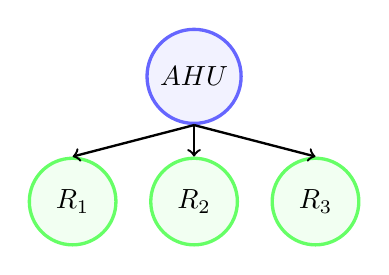
\begin{tikzpicture}[
                    racknode/.style={circle, draw=green!60, fill=green!5, very thick, minimum size=1.1cm},
                    ahunode/.style={circle, draw=blue!60, fill=blue!5, very thick, minimum size=5mm},
                ]
                    %Nodes
                    \node[ahunode](ahu){$AHU$};
                    \node[racknode](rack1)[below=0.4cm of ahu] {$R_2$};
                    \node[racknode](rack2)[right=0.4cm of rack1] {$R_3$};
                    \node[racknode](rack3)[left=0.4cm of rack1] {$R_1$};

                    %Lines
                    \draw[line width=0.3mm, ->](ahu.south) -- (rack3.north);
                    \draw[line width=0.3mm, ->](ahu.south) -- (rack1.north);
                    \draw[line width=0.3mm, ->](ahu.south) -- (rack2.north);
                \end{tikzpicture}
            \end{subfigure}\hfill
            \begin{subfigure}[b]{0.3\textwidth}
                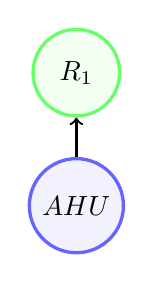
\begin{tikzpicture}[
                    racknode/.style={circle, draw=green!60, fill=green!5, very thick, minimum size=1.1cm},
                    ahunode/.style={circle, draw=blue!60, fill=blue!5, very thick, minimum size=5mm},
                ]
                    %Nodes
                    \node[ahunode](ahu){$AHU$};
                    \node[racknode](rack3)[above=0.5cm of ahu] {$R_1$};

                    %Lines
                    \draw[line width=0.3mm, ->](ahu.north) -- (rack3.south);
                \end{tikzpicture}
            \end{subfigure}\\
            \begin{subfigure}[b]{0.45\textwidth}
                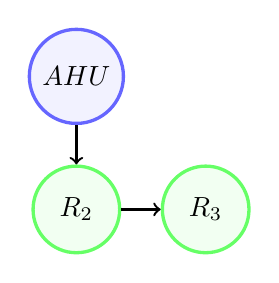
\begin{tikzpicture}[
                    racknode/.style={circle, draw=green!60, fill=green!5, very thick, minimum size=1.1cm},
                    ahunode/.style={circle, draw=blue!60, fill=blue!5, very thick, minimum size=5mm},
                ]
                    %Nodes
                    \node[ahunode](ahu){$AHU$};
                    \node[racknode](rack1)[below=0.5cm of ahu] {$R_2$};
                    \node[racknode](rack2)[right=0.5cm of rack1] {$R_3$};

                    %Lines
                    \draw[line width=0.3mm, ->](ahu.south) -- (rack1.north);
                    \draw[line width=0.3mm, ->](rack1.east) -- (rack2.west);
                \end{tikzpicture}
            \end{subfigure}\hfill
            \begin{subfigure}[b]{0.45\textwidth}
                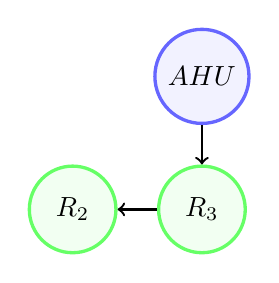
\begin{tikzpicture}[
                    racknode/.style={circle, draw=green!60, fill=green!5, very thick, minimum size=1.1cm},
                    ahunode/.style={circle, draw=blue!60, fill=blue!5, very thick, minimum size=5mm},
                ]
                    %Nodes
                    \node[ahunode](ahu){$AHU$};
                    \node[racknode](rack2)[below=0.5cm of ahu] {$R_3$};
                    \node[racknode](rack1)[left=0.5cm of rack2] {$R_2$};

                    %Lines
                    \draw[line width=0.3mm, ->](ahu.south) -- (rack2.north);
                    \draw[line width=0.3mm, ->](rack2.west) -- (rack1.east);
                \end{tikzpicture}
            \end{subfigure}
         \end{figure}
    \end{columns}
\end{frame}

\begin{frame}
    \frametitle{HRF EO6 predictions}
    \begin{figure}
        \includegraphics<1>[scale=0.7]{images/comp_eo6_1}
        \includegraphics<2>[scale=0.7]{images/comp_eo6}
    \end{figure}
\end{frame}

\begin{frame}
    \frametitle{HRF Q8 predictions}
    \begin{figure}
        \includegraphics<1>[scale=0.7]{images/comp_q8_1}
        \includegraphics<2>[scale=0.7]{images/comp_q8}
    \end{figure}
\end{frame}

\begin{frame}
    \frametitle{HRF QQplots}
    \begin{figure}
        \includegraphics<1>[scale=0.7]{images/simple_hrf_qqplot_eo6}
        \includegraphics<2>[scale=0.7]{images/simple_hrf_qqplot_q8}
    \end{figure}
\end{frame}

\begin{frame}
    \frametitle{HRF Simulation}
    \begin{figure}
        \includegraphics<1>[scale=0.33]{images/heatapp_hrf_2_t0}
        \includegraphics<2>[scale=0.33]{images/heatapp_hrf_2_t1}
        \includegraphics<3>[scale=0.33]{images/heatapp_hrf_2_t4}
        \includegraphics<4>[scale=0.33]{images/heatapp_hrf_2_t8}
    \end{figure}
\end{frame}

\begin{frame}
    \frametitle{Questions}
    \center{Questions ?}
\end{frame}

\end{document}
